\chapter{User Study}
\label{ch:user-study}

\section{Hypothesis and Objective}
\label{sec:hypothesis}

This chapter addresses the final research question: \emph{R3: What is the user acceptance and usability of a passwordless document encryption system?} In order to assess the usability and user acceptance of the passwordless document encryption system we developed, we conducted an IRB-approved human subjects research study. We hypothesized that using the passwordless approach to encrypt and share documents would result in an easier and more enjoyable experience for participants when compared to using a traditional password-based encryption approach (such as is used by Adobe Acrobat or Microsoft Word) for protecting sensitive documents. Specifically our research study hypothesis was as follows:

\begin{itemize}
    \item Passwordless document encryption using modern authentication (passkeys, biometrics, YubiKeys) will provide a superior sense of security, greater usability, and a perceived better level of deployability compared to traditional password-based encryption.
    \item Improved usability of document encryption tools will lead to increased adoption and a sense of stronger security practices.
    \item Users will trust and prefer passwordless encryption methods over traditional password-based approaches.
\end{itemize}

In short, our objective was to assess user acceptance and usability through comparative testing of the passwordless and password-based document encryption process.

\section{Procedure}
\label{sec:procedure}

The study design was modeled after two similar FIDO2 usability studies~\cite{lyastani_fido2_2020,wursching_fido2_2023}. The IRB-approved study was a within-groups lab experiment where users performed the tasks of encryption, decryption, and sharing on two similar online platforms: one password-based document encryption tool and one passwordless document encryption tool. Participants responded to the System Usability Scale (SUS) and Van Der Laan User Acceptance Scale after using each system and then gave comments about their experience in response to semi-structured interview questions. An overview of the study procedure is shown in Figure~\ref{fig:procedure}.

% Study Procedure Diagram — TikZ version
\begin{figure}[htbp]
    \centering
    % Resizebox ensures this wide diagram fits perfectly within page margins
    \resizebox{\textwidth}{!}{%
    \begin{tikzpicture}[
        node distance=0.5cm,
        % Clean, minimalist academic style
        stage/.style={
            rectangle, rounded corners=2pt, minimum width=2.0cm, minimum height=1.3cm,
            text centered, font=\footnotesize, text width=1.8cm,
            draw=black!80, thick, fill=white
        },
        % Faint gray for bookend stages to make the core tasks pop
        neutral/.style={stage, fill=gray!10},
        systemA/.style={stage},
        systemB/.style={stage},
        arrow/.style={->, >=stealth, thick, draw=black!60},
        stagenum/.style={font=\small\bfseries, text=black},
        % Increased text width to 2.4cm so "Encrypt, Decrypt," fits on one line
        sublabel/.style={font=\scriptsize\itshape, text=black!70, text width=2.4cm, align=center},
    ]

    % Nodes
    \node[neutral]  (s1) {Screening\\Survey};
    \node[neutral]  (s2) [right=of s1] {Consent \&\\Briefing};
    \node[systemA]  (s3) [right=of s2] {Tasks\\System A};
    \node[systemA]  (s4) [right=of s3] {SUS + VdL\\System A};
    \node[systemB]  (s5) [right=of s4] {Tasks\\System B};
    \node[systemB]  (s6) [right=of s5] {SUS + VdL\\System B};
    \node[neutral]  (s7) [right=of s6] {Interview};

    % Arrows
    \foreach \i/\j in {s1/s2, s2/s3, s3/s4, s4/s5, s5/s6, s6/s7} {
        \draw[arrow] (\i) -- (\j);
    }

    % Stage numbers
    \foreach \i/\n in {s1/1, s2/2, s3/3, s4/4, s5/5, s6/6, s7/7} {
        \node[stagenum, below=0.15cm of \i] {\n};
    }

    % Sublabels
    \node[sublabel, below=0.55cm of s1] {Demographics,\\ATI, PC};
    \node[sublabel, below=0.55cm of s2] {In-person with\\researcher};
    \node[sublabel, below=0.55cm of s3] {Encrypt, Decrypt,\\Share};
    \node[sublabel, below=0.55cm of s5] {Encrypt, Decrypt,\\Share};
    \node[sublabel, below=0.55cm of s7] {Audio recorded,\\10 questions};

    % Counterbalance bracket
    \draw[decorate, decoration={brace, amplitude=5pt, raise=4pt}, draw=black!70, thick]
        (s3.north west) -- (s6.north east)
        node[midway, above=10pt, font=\footnotesize\itshape, text=black!80] 
        {Counterbalanced order};

    \end{tikzpicture}%
    } % End resizebox
    \caption{Overview of the study procedure.}
    \label{fig:procedure}
\end{figure}


Participants first completed a screening survey, consent acknowledgement, and responded to background questions to understand their basic demographics, familiarity with sensitive documents, and experience with passwordless authentication (What is your age?, What is your job/industry?, How often do you work with electronic documents that contain sensitive or controlled information?, Have you had experience with passwordless authentication?).

Additionally, participants completed the Affinity for Technology Interaction (ATI) Scale and the Privacy Concern (PC) Scale (described in Sections~\ref{sec:pc-scale} and~\ref{sec:ati-scale}). These factors---technical background, affinity for technology, and privacy concerns---have been shown to influence user perceptions of new technologies~\cite{lyastani_fido2_2020,wursching_fido2_2023}.

After completing the screening, consent, and background questions, participants then met in-person with a researcher who asked them to imagine themselves in a corporate environment with sensitive information. Using scenario-based storytelling and a controlled lab environment gave narrative context and helped subjects be in the mindset of ``work'' without introducing the risk of using real sensitive files of the participant. Participants used their own laptop computer and/or mobile phone (bring-your-own-device, BYOD) so their browser, password managers, browser extensions, and operating system settings would feel accurate to their typical tools and configurations.

Users often struggle with FIDO2 because they don't understand it. As part of the study procedures we asked about the participant's experience with multi-factor authentication and included an optional short video explaining how passkeys work. This aimed to help reduce the possibility of measuring the lack of knowledge about passwordless methods rather than the usability of the passwordless system which would be present if users did not understand the foundational concepts or were confused about it. The researcher answered basic clarifying questions prior to beginning the system evaluations.

The study was a counter-balanced within-groups lab experiment where each participant used and evaluated both systems. The two systems were the Adobe Acrobat Online Document Encryption website (available at: \url{www.adobe.com/acrobat/online/password-protect-pdf.html}) and the passwordless document encryption tool designed and developed during this research which was described in Chapter~\ref{ch:system-design} (available at: \url{https://doc-protect.vercel.app}). Both systems were accessed by the participants through their web browser on their laptop computer or mobile device. All sessions were conducted in-person either individually with a researcher or in small group sessions (2--5 participants together). Each participant was randomly assigned an order for which platform to evaluate first. This was done in an effort to reduce learning bias.

The set of tasks was nearly identical for both systems and consisted of three steps: encrypt a file, decrypt the file, share the file. The files were shared with the researcher conducting the study session so that the password could be communicated directly as needed. The complete task instructions provided to participants for each system are included in Appendix~\ref{ap:instruments}.

After completing each task set on a system, the participant would fill out the SUS and Van Der Laan scales to measure usability and user acceptance of the system. These were presented as multiple choice questions in a Qualtrics survey. Once the scales were completed for the first system participants would then continue to the next system where they would complete the tasks and then respond to the same scales for the second system they used.

Once each participant completed the tasks on both systems and responded to the SUS and VdL scales for each system, the researcher would confirm consent to begin audio-recording and then record the participant's responses to semi-structured interview questions. The 10 interview questions used are included in Appendix~\ref{ap:instruments}. In total, each participant spent 35--45 minutes, consisting of 5--10 minutes on the screening, consent, and background, 20--25 minutes using and evaluating the two systems, and 5--10 minutes responding to the interview questions.

The research study was presented to the University Institutional Review Board (IRB) which reviewed the study plan and concluded that the study was exempt from full review as subjects were de-identified, data protected, and the study posed minimal to no risk to subjects.\footnote{BYU IRB number 2026-028.}

\section{Participants}
\label{sec:participants}

A sample of 21 participants was selected as appropriate for an initial exploratory study combining quantitative scales with qualitative interviews. A within-subjects design was chosen to maximize statistical power given the sample size (N=21), as each participant evaluated both systems and served as their own control. While a between-subjects design (where participants only see one method, not both) would help avoid contrast effects (where users judge a new technology by comparing it to a familiar one rather than on its own merits) this was not feasible with this sample size. To mitigate ordering and learning effects, the study used counterbalanced assignment: participants were randomly assigned to complete the password-based tasks first or the passwordless tasks first, so that any learning or fatigue effects were distributed evenly across conditions. This meant each user had a random chance of first seeing the passwordless system or first seeing the password based method.

Participants were recruited through personal contact, word of mouth, classroom announcements (including digital announcements), social media (e.g., LinkedIn, Facebook), and flyers. The recruitment materials are attached in Appendix~\ref{ap:recruitment}.

Participants were screened to identify adults over 18 who were able to meet in-person for the study, with a variety of ages, education status, and computer science backgrounds. In the Qualtrics screening survey one question asked about age (How old (in years) are you?) and automatically screened out individuals who were under 18. Another question in the Qualtrics survey asked if participants were able and willing to meet in person for the research study. No vulnerable populations were involved in the research study. No compensation was provided. All research activities were performed in English.

\begin{table}[htbp]
    \centering
    \begin{threeparttable}
        \caption{Participant Demographics}
        \label{tab:demographics}
        \begin{tabular}{ll}
            \toprule
            \textbf{Variable} & \textbf{Sample ($N = 21$)} \\
            \midrule
            \textbf{Gender} & \\
            \quad Male & 76.2\% (16) \\
            \quad Female & 23.8\% (5) \\
            \addlinespace
            \textbf{Age} & $M = 29.2, SD = 11.7$ \\
            \quad 18--24 & 38.1\% (8) \\
            \quad 25--34 & 47.6\% (10) \\
            \quad 35--44 & 0.0\% (0) \\
            \quad 45--54 & 4.8\% (1) \\
            \quad 55--64 & 9.5\% (2) \\
            \addlinespace
            \textbf{Education} & \\
            \quad High school graduate & 4.8\% (1) \\
            \quad Some college & 19.0\% (4) \\
            \quad Bachelor's degree & 66.7\% (14) \\
            \quad Master's degree & 4.8\% (1) \\
            \quad Doctorate & 4.8\% (1) \\
            \addlinespace
            \textbf{Technical background} & \\
            \quad Yes & 71.4\% (15) \\
            \quad No & 28.6\% (6) \\
            \addlinespace
            \textbf{ATI} (1--6; $\alpha = .893$) & $M = 4.11, SD = 0.91$ \\
            \addlinespace
            \textbf{Privacy Concerns} (1--7; $\alpha = .803$) & $M = 5.58, SD = 1.01$ \\
            \bottomrule
        \end{tabular}
        \begin{tablenotes}
            \small
            \item \textit{Note:} ATI = Affinity for Technology Interaction (Franke et al., 2019); higher scores indicate greater technology affinity. Privacy Concerns Scale (Langer, König \& Fitili, 2018); higher scores indicate greater concern about data privacy. Technical background = self-reported computer science or cybersecurity education or professional experience.
        \end{tablenotes}
    \end{threeparttable}
\end{table}


The demographic profile of the participants (N=21) is summarized in Table~\ref{tab:demographics}. The sample skewed heavily male (76.2\%) and was relatively young ($M=29.2$, $SD=11.7$). A large majority of the participants (71.4\%) possessed a formal technical background (e.g., university study or professional experience in Computer Science or Cybersecurity).

Each participant was assigned a unique ID (e.g., P01, P02) which was not derived from any personal information. This unique ID was used in place of any personally identifying information for data storage and analysis. Participant IDs are non-sequential due to the exclusion of pilot testers and incomplete responses during data collection.

\section{Instruments}
\label{sec:instruments}

A mixed-methods process combining quantitative scales and qualitative interview questions was used to assess the factors in this study. Prior to the usability session, each participant completed the Privacy Concern (PC) Scale and Affinity for Technology Interaction (ATI) Scale. During the session, each participant completed the System Usability Scale (SUS) and the Van der Laan System Acceptance Scale (VdL) for each of the two encryption methods. These instruments were used to determine scores for the usability and acceptance of the two systems and understand which factors impacted user perceptions. At the conclusion of the session, qualitative responses were gathered by an audio-recorded semi-structured interview (5--10 minutes, 10 questions). Together, these instruments captured quantitative and qualitative data during the experiment.

\subsection{Privacy Concerns Scale (PC)}
\label{sec:pc-scale}

The Privacy Concern Scale~\cite{langer_information_2018} is a four-item instrument that measures an individual's general concerns about whether novel technologies threaten personal privacy. Because document encryption is a domain where privacy sensitivity may influence user perceptions, this scale was included to measure and observe the potential impact of privacy concern as a covariate. The scale was developed by Langer et al.~\cite{langer_information_2018} in a study examining reactions to novel technology and has since been used in multiple passwordless authentication usability studies, including Lyastani et al.~\cite{lyastani_fido2_2020} and W\"ursching et al.~\cite{wursching_fido2_2023}. Each participant completed the scale once prior to the study session.

\subsection{Affinity for Technology Interaction Scale (ATI)}
\label{sec:ati-scale}

The Affinity for Technology Interaction (ATI) Scale~\cite{franke_personal_2019} is a nine-item instrument that measures how much an individual likes to engage with technical systems. Because an interest in technology can bias user perceptions and usability ratings of novel systems, the ATI was included to measure and account for this factor in the analysis. The scale has been independently validated with excellent reliability ($\omega = .90$) and construct validity~\cite{lezhnina_multimethod_2020}. Each participant completed the ATI once prior to the study session.

\subsection{System Usability Scale (SUS)}
\label{sec:sus-scale}

The System Usability Scale (SUS) is an industry-standard, validated instrument used to measure the perceived usability of a system~\cite{brooke_sus_1996}. It consists of 10 items and produces a single overall unit of measure on a 0--100 scale, enabling comparison against established benchmarks (see Figure~\ref{fig:sus-framework}).

\begin{figure}[htbp]
    \centering
    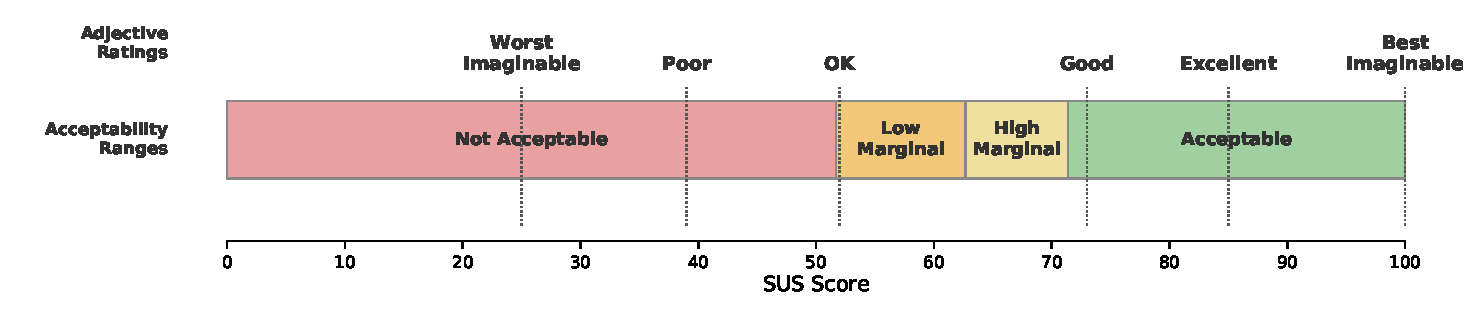
\includegraphics[width=5in]{figures/sus-benchmark-scale.pdf}
    \caption[SUS score interpretation framework.]{SUS score interpretation framework showing adjective ratings and acceptability ranges. Adapted from Bangor, Kortum, and Miller~\cite{bangor_determining_2009}.}
    \label{fig:sus-framework}
\end{figure}

The scores of individual questions within the SUS are not meant to be considered or evaluated individually as the SUS calculations work together to produce a single composite score of the overall system usability~\cite{brooke_sus_1996}. The SUS was selected for its simplicity, broad adoption, and well-established validity. Reliability analyses have consistently reported coefficient alphas at or above .90~\cite{lewis_item_2018,bangor_empirical_2008,sauro_correlations_2009}, and the scale has been widely adopted across both industry and academic research~\cite{lewis_item_2018}. In this study, each participant completed the SUS once for the password-based method and once for the passwordless method, allowing a within-subjects comparison of perceived usability.

\subsection{Van der Laan System Acceptance Scale (VdL)}
\label{sec:vdl-scale}

The Van der Laan System Acceptance Scale~\cite{vanderlaan_simple_1997} is a nine-item instrument that measures user acceptance of new technologies. Each item is rated on a five-point scale. The scale has traditionally been described as comprising two subscales---usefulness and satisfaction---though subsequent factor analyses have debated this structure; for example, Schmid~\cite{schmid_tas_2022} found evidence for a one-factor solution using Bayesian exploratory factor analysis. While most commonly used in transportation research, the scale has been applied in technology usability studies as a simple and efficient measure of acceptance. In this study, participants completed the Van der Laan scale for each encryption method to compare acceptance between the password-based and passwordless approaches.

\subsection{Semi-Structured Interviews}
\label{sec:interviews}

At the conclusion of each study session, participants responded to semi-structured interview questions. Ten open-ended questions were used to gather feedback on their experience using each of the encryption methods, their current practices with sensitive documents, their willingness to adopt the passwordless method, as well as suggestions for improvement and the advantages or disadvantages they perceived in each method. The full interview protocol is included in Appendix~\ref{ap:instruments}. Interviews were conducted individually or in small groups (two to five participants) depending on the session.

\section{Data Processing}
\label{sec:data-processing}

Responses were collected through Qualtrics, which recorded each participant's raw Likert-scale responses for both systems. The survey was structured with two blocks: the first block captured SUS (10 items, 1--5 scale) and VdL (9 items, 1--5 semantic differential) responses for whichever system the participant used first, and the second block captured the same instruments for the second system. A data field recorded the counterbalanced presentation order, enabling the responses to be correctly assigned to the password-based or passwordless condition regardless of which was administered first.

SUS scores were computed following Brooke's (1996) standard procedure: for odd-numbered items, the score contribution is the scale position minus 1; for even-numbered items, the contribution is 5 minus the scale position. The sum of the 10 item contributions is multiplied by 2.5 to produce a score on a 0--100 scale. Van der Laan scores were converted from the raw 1--5 Likert responses to the standard $-2$ to $+2$ scale, with polarity reversals applied to items where the positive pole appeared first in the semantic differential pair. The five usefulness items (1, 3, 5, 7, 9) and four satisfaction items (2, 4, 6, 8) were then averaged into their respective subscale scores. All scoring and statistical analysis was performed using a Python processing script. The complete per-participant scored data is provided in Appendix~\ref{ap:data}.
